% article or report works
\documentclass[letterpaper,12pt]{article}

% language and font encodings
\usepackage[english]{babel}

% page size and margins (choose one: two general options)

%% \setlength{\evensidemargin}{0in}
%% \setlength{\oddsidemargin}{0.5in}
%% \setlength{\textwidth}{6in}
%% \setlength{\topmargin}{0.2in}
%% \setlength{\textheight}{8.6in}
%% \setlength{\footnotesep}{14pt}

\usepackage[letterpaper, top=2cm, bottom=2cm, left=2cm, right=2cm, marginparwidt=1.75cm]{geometry}
\setlength {\marginparwidth}{2cm}

% useful packages
\mathchardef\mhyphen="2D
\usepackage{graphicx}
\usepackage{tabularx}
\usepackage{array}
\usepackage[colorinlistoftodos]{todonotes}
\usepackage[colorlinks=true, allcolors=blue]{hyperref}
\usepackage{enumitem}
\usepackage{marginnote}
\usepackage{mathtools}
\usepackage[normalem]{ulem}
\usepackage[utf8]{inputenc}
\usepackage{fancyhdr}
\usepackage{booktabs}
\usepackage{enumitem}
\usepackage{caption}
\usepackage{amsmath,amsthm,amssymb,amsfonts}
\usepackage{physics}

% theorem types
\newtheorem{theorem}{Theorem}[section]
\newtheorem{lemma}[theorem]{Lemma}
\newtheorem{corollary}[theorem]{Corollary}
\newtheorem{conjecture}[theorem]{Conjecture}
\newtheorem{proposition}[theorem]{Proposition}
\newtheorem*{uconj}{Uniform Boundedness Conjecture}
\theoremstyle{definition}
\newtheorem{definition} [theorem] {Definition}
\newtheorem{claim}[theorem]{Claim}
\newtheorem{example} [theorem] {Example}
\newtheorem{remark} [theorem] {Remark}

% plotting and graphing using tikz
\usepackage{pgfplots}
\pgfplotsset{compat=1.18} % only compatible with the current version of pgfplots installed
\usepackage{mathrsfs}
\usepackage{tikz}

% only use if tikzit is used; two essential files are needed along with this to work
%% \usepackage{tikzit}
%% \input{default.tikzstyles}

% user-defined macros
\newcommand{\C}{{\mathbb{C}}}
\newcommand{\F}{{\mathbb{F}}}
\newcommand{\N}{{\mathbb{N}}}
\newcommand{\Q}{{\mathbb{Q}}}
\newcommand{\PP}{{\mathbb{P}}}
\newcommand{\R}{{\mathbb{R}}}
\newcommand{\Z}{{\mathbb{Z}}}

\newcommand{\cK}{{\mathcal{K}}}

\newcommand{\fm}{{\mathfrak{m}}}
\newcommand{\fo}{{\mathfrak{o}}}

\newcommand{\Cp}{\C_p}
\newcommand{\Cv}{\C_v}
\newcommand{\Qp}{\Q_p}
\newcommand{\Qpbar}{\bar{\Q}_p}
\newcommand{\Dbar}{\overline{D}}

% user-defined math operators
\DeclareMathOperator{\rad}{rad}
\DeclareMathOperator{\diam}{diam}
\DeclareMathOperator{\divop}{div}

\begin{document}

\begin{titlepage}

  \begin{center}

    \vspace*{\fill}

    \vspace*{0.5cm}

    \huge{Arc Length Contest}

    \vspace*{0.5cm}

    \large{Henry Yu}

    \vspace*{\fill}

  \end{center}

\end{titlepage}

\newpage

\raggedright

\section*{Solution}

The most logical solution (to me) to obtain the shortest arc length following these requirements seemed to be a half ellipse extending from 0 to 1.
\newline
Recall that the formula for an ellipse is

\begin{center}
    $\dfrac{x^2}{a^2}\,+\dfrac{y^2}{b^2}\,=\,1$.
\end{center}

Simplifying to get the equation in terms of y,

\begin{center}
    $\dfrac{y^2}{b^2}\,=\,1\,-\,\dfrac{x^2}{a^2}$
    \vskip 16pt
    $y^2\,=\,b^2\,-\,\dfrac{x^2b^2}{a^2}$
    \vskip 16pt
    $y\,=\,\sqrt{b^2\,-\,\dfrac{x^2b^2}{a^2}}$
    \vskip 16pt
    \hspace{5.5cm}$y\,=\,b\,\sqrt{1\,-\,\dfrac{x^2}{a^2}}$. \hspace{5cm}(1)
\end{center}

Since we are only looking for half of an ellipse, the area is cut in half:

\begin{center}
    $\dfrac{1}{2}\pi ab\,=\,1$.
\end{center}

Since one of the requirements states that $f(0)\,=\,f(1)\,=\,0$,

\begin{center}
    $2a\,=\,1$.
\end{center}

Solving for a and b:

\begin{center}
    $a\,=\,\dfrac{1}{2}$
    \vskip 16pt
    $b\,=\,\dfrac{\pi}{4}$.
\end{center}

Substituting a and b into (1), we obtain the new equation:

\begin{center}
    $y\,=\,\dfrac{4}{\pi}\,\sqrt{1\,-\,4\left(x\,-\,\dfrac{1}{2}\right)^2}$.
\end{center}

\pagebreak

The area of the previous equation is determined by the following equation:

\begin{center}
    $\int_{0}^{1} f(x)\,dx$.
\end{center}

After evaluating the integral for our specific case, we determine that the area is indeed 1, satisfying the requirements.

The arc length of the previous equation is determined by the following equation:

\begin{center}
    $\int_{0}^{1} \sqrt{1\,+\,\left(\dfrac{dy}{dx}\right)^2}\,dx$.
\end{center}

After finding the derivative of (1) to be

\begin{center}
    $-\dfrac{16x-8}{{\pi}\sqrt{1-4\left(x-\dfrac{1}{2}\right)^2}}$,
\end{center}

we evaluate the arc length formula to find that the arc length for this function equals 2.919462643547631.

\begin{center}
    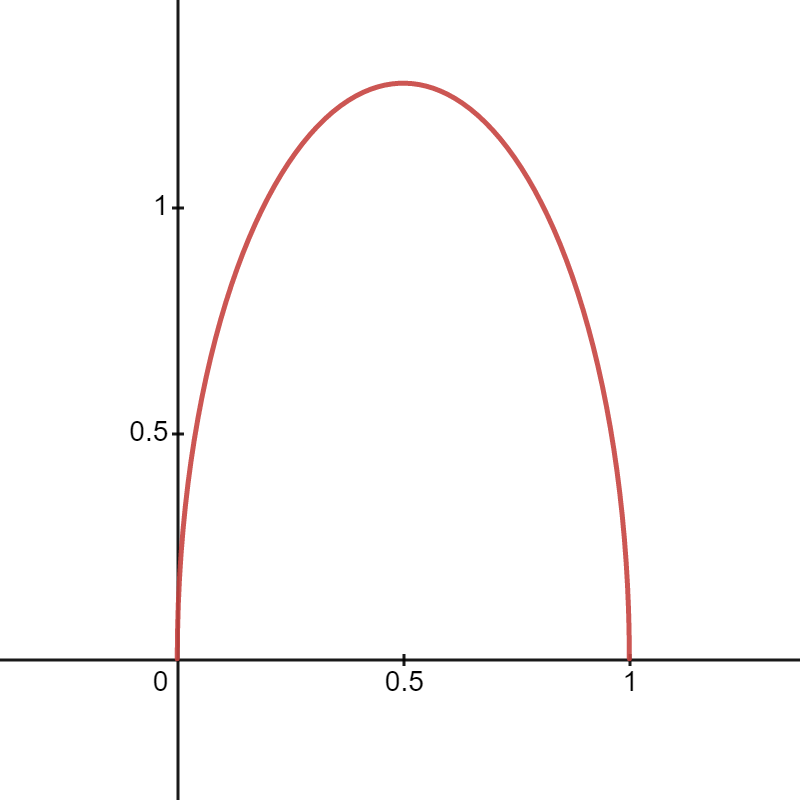
\includegraphics[scale=0.3]{halfellipse.png}
\end{center}

\pagebreak

\section*{Other Possible Solution}

After looking over the graph, I realized that to get a better answer, the curves should become relatively straighter and perhaps looking somewhat like this instead:

\begin{center}
    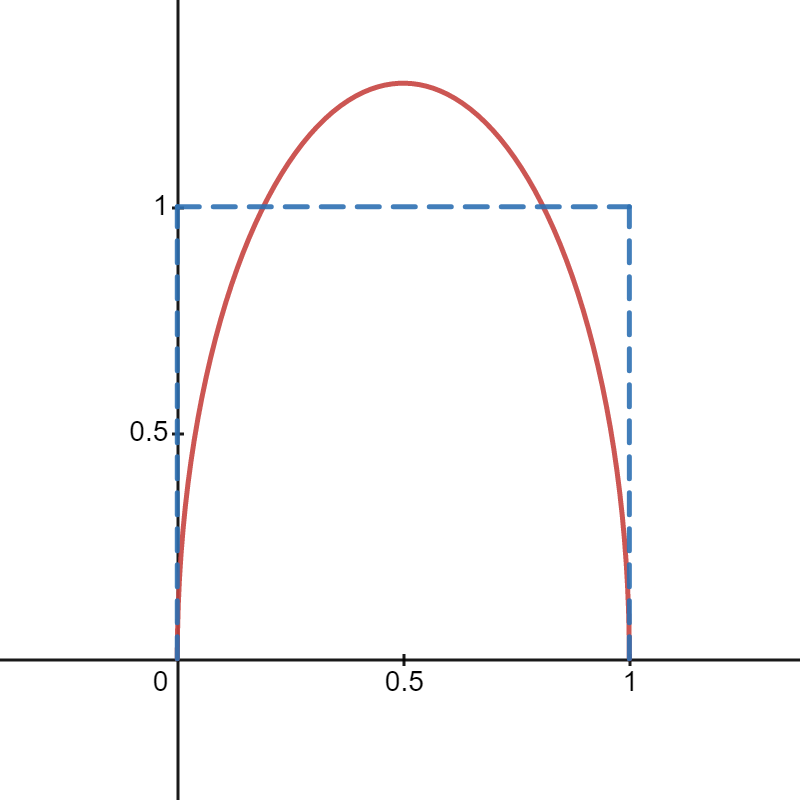
\includegraphics[scale=0.3]{projection.png}
\end{center}

This reminded me of superellipses, so after finding my half ellipse solution, I attempted to solve this problem using superellipses instead.
\newline
Recall that the formula for a superellipse is

\begin{center}
    $\abs{\,\dfrac{x}{a}\,}^n\,+\,\abs{\,\dfrac{y}{b}\,}^n\,=\,1$.
\end{center}

Solving for y,

\begin{center}
    $\abs{\,\dfrac{y}{b}\,}^n\,=\,1\,-\,\abs{\,\dfrac{x}{a}\,}^n$
    \vskip 16pt
    $\abs{\,\dfrac{y}{b}\,}=\,\left(1\,-\abs{\,\dfrac{x}{a}\,}^n\right)^{1/n}$
    \vskip 16pt
    $\dfrac{y}{b}\,=\,\pm\,\left(1\,-\abs{\,\dfrac{x}{a}\,}^n\right)^{1/n}$
    \vskip 16pt
    $y\,=\,\pm\,b\,\left(1\,-\abs{\,\dfrac{x}{a}\,}^n\right)^{1/n}$.
\end{center}

\pagebreak

Setting the variable a equal to 1/2 like during the ellipse solution, we find that the equation becomes

\begin{center}
    $y\,=\,\pm\,b\,\left(1\,-\abs{\,2x\,}^n\right)^{1/n}$.
\end{center}

We then shift the graph to the right by one unit because the graph currently goes from $x\,=\,-0.5$ to $x\,=\,0.5$:

\begin{center}
    $y\,=\,\pm\,b\,\left(1\,-\abs{\,2x\,-\,1\,}^n\right)^{1/n}$.
\end{center}

We also only want positive values for y, so the negative sign is removed:

\begin{center}
    \hspace{4.6cm}$y\,=\,b\,\left(1\,-\abs{\,2x\,-\,1\,}^n\right)^{1/n}$.\hspace{4.6cm}(2)
\end{center}

We wish to find a general solution for b:

\begin{center}
    $\int_{0}^{1} f(x)\,dx\,=1$
    \vskip 16pt
    $\int_{0}^{1} b\,\left(1\,-\abs{\,2x\,-\,1\,}^n\right)^{1/n}\,dx\,=1$
    \vskip 16pt
    $b\int_{0}^{1}\left(1\,-\abs{\,2x\,-\,1\,}^n\right)^{1/n}\,dx\,=1$
    \vskip 16pt
    $b\,=\,\dfrac{1}{\int_{0}^{1}\left(1\,-\abs{\,2x\,-\,1\,}^n\right)^{1/n}}\,dx$.
\end{center}

We wish to push n to infinity while keeping b equal to the reciprocal of the integral of $\left(1\,-\abs{\,2x\,-\,1\,}^n\right)^{1/n}$ so that the area under the curve stays at 1.

\begin{center}
    $\lim\limits_{n \to \infty} b\,\left(1\,-\abs{\,2x\,-\,1\,}^n\right)^{1/n}\,=$ arc length $\{b\,=\,\dfrac{1}{\int_{0}^{1}\left(1\,-\abs{\,2x\,-\,1\,}^n\right)^{1/n}}\,dx\}$.
\end{center}


I went with $n\,=\,4$ since that was the absolute furthest I could push the calculator to find a value when finding the arc length without a b value.

Using $n\,=\,4$, we find that b equals

\begin{center}
    $b\,=\,\dfrac{1}{\int_{0}^{1}\left(\,1\,-\abs{\,2x\,-\,1\,}^4\right)^{1/4}}\,dx$.
\end{center}

Solving for b, we find that b $\approx$ 1.078314317.

\pagebreak

The final equation is

\begin{center}
    $y\,=\,1.078314317\,\left(1\,-\abs{\,2x\,-\,1\,}^4\right)^{1/4}$.
\end{center}

Solving for area, we find that it is off by 4/10000 from 1, most likely from some rounding but close enough to safely assume it equals 1.

Solving for arc length, we find that it equals 2.810352052463713.

\begin{center}
    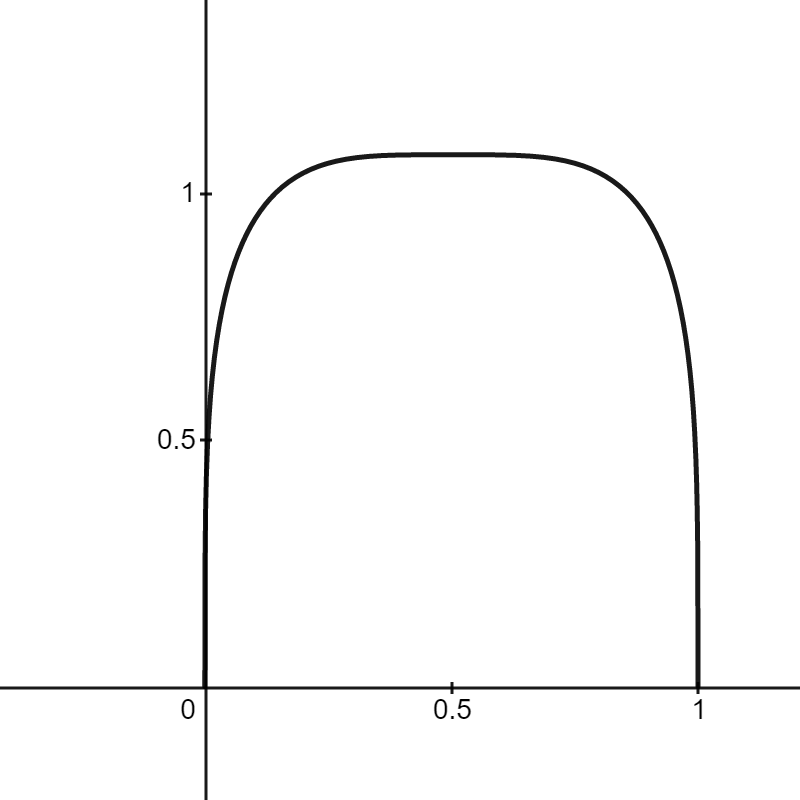
\includegraphics[scale=0.3]{superellipse.png}
\end{center}

\end{document}